\documentclass{article}
\usepackage[margin=1in]{geometry}
\usepackage{graphics}
\usepackage{tikz}
\usepackage{../common}
\usepackage{../pagesetup}

\begin{document}
%\lecture{**LECTURE-NUMBER**}{**DATE**}{**LECTURER**}{**SCRIBE**}
\lecture{18}{November 8}{Sasha Rush} {Jeff Chang, Michael Els, Zhixian Lei, Yuting Sun, Xincheng You, Srivatsan Srinivasan}{Variational Auto-encoders and GANs}%% Add your scribe names!!

Today we are going to go a step forward in Variational Inference. We are going to combine the variational inference and neural networks. 
\subsection{Autoencoder}
Suppose we receive a signal $x$ from a source. Then we encode $x$ with encoding function $Enc$
$$ z = Enc(x) $$
so that $z$ is simpler than $x$, for example, $z$ can be lower dimension than $x$ or the learned encoding function itself can be a simple function. The goal is to limit the capacity of the model by parameterising $enc$ and $p()$, and to learn them from the data. This leads to the model learning the optimal compression for the data which only saves the most important information and discards the rest. This encoding is often nonlinear in practice, for example, people often use neural networks. Then $z$ might be changed to $z'$ by noise. After that, we want to recover $x$ by inference:
$$ \hat{x} = \textrm{argmax}_{x'}\Pr(x = x'|z') $$
This is basically what autoencoder does. For variational autoencoder, we need to parameterize function $Enc$ and $\Pr(x = x'|z')$ usually with neural networks. We might want to learn these functions from data. \\
\centerline{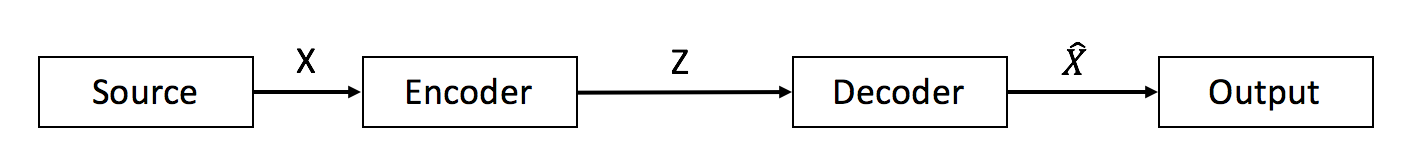
\includegraphics[width=13cm]{chart.png}}
\subsection{Back to Variational Inference}
\begin{eqnarray}
\log p(x) & = &\log \int_{\theta} p(\theta)p(x | \theta)d\theta \\
& = & \log \int_{\theta}q(\theta)(p(\theta)/q(\theta))p(x|\theta)d\theta \\
& \geq & E_q\left[\log \frac{p(\theta)}{q(\theta)}p(x|\theta)\right] \\
& = & -\textrm{KL}(q(\theta)|p(\theta)) + E_q[\log p(x|\theta)]
\end{eqnarray}
where the first term makes $q$ close to prior $p$ and the second term is the likelihood based on $q$.
There are two methods to optimization above expression
\begin{itemize}
\item Coordinates Ascent (CAVI)
\item Stochastic Gradient Descent (SGD)
\end{itemize}
where CAVI is the method we have introduced in previous lectures and SGD is just directly optimize this function.

About the choice of $q$-function, we have following several methods:
\begin{itemize}
\item We can make mean field assumption (which requires the full Markov blanket), then $q(\theta) = \prod_i q_i(\theta)$
\item We can also do structured mean field. Basically we can divide this graph into several simple subgraphs (they can overlap each other). Inside each subgraphs we can do belief propagation using for example forward-backward algorithm and outside of the subgraphs we use mean field approximation. This $q$ is closer to the original and has a better bound.
\item More generally we can use neural networks, where $\lambda$ are neural network parameters and we use $q_\lambda$ to approximate the posterior. 
\end{itemize}
\subsection{Variational Autoencoder}
We have learned many models in this class. The Ising model is an example that is difficult to do inference on. There are also models that we can't use EM on. An example of such a model is illustrated here: \\

\begin{center}
\begin{tikzpicture}
    %Define nodes
    \node[latent](x){$x$};
    \node[latent, above=of x](z){$z$};
    \node[latent, above right=of x](mu){$\mu$};
    
    \edge {mu} {z};
    \edge {mu} {x};
    \edge {z} {x};
    
    \plate {zx} {(z)(x)} {$N$};
    
\end{tikzpicture}
\end{center}
Since the parameters are not fixed, the EM fails in this case. Using this as a motivating example, let's examine Variational Autoencoders. In our previous examples for inference, we always consider the conditional distribution as discrete distribution or just linear Gaussian distribution, and that we can calculate our posterior in a straightforward manner. But in general $p(\textrm{Data}|\textrm{Label})$ can be non-linear, for example, neural network. Then $p(\textrm{Label}|\textrm{Data})$ becomes intractable. In this case, we should make $q$-function as a neural network. Suppose $z$ are labels, $x$ are data and $\mu$ are parameters. 
And we assume
$$\Pr(x | z, \mu) = \textrm{softmax}(w\phi(x; \mu))$$
where $\phi$ is a neural network. We use neural networks to compute $q$ functions
$$ q_{\lambda}(z) = \mathcal{N}(w^1\phi_1(x; \lambda), w^2\phi_2(x; \lambda)) $$
where $\phi_1$ and $\phi_2$ are neural networks. $w^1$ and $w^2$ are transformation parameters. 

We can interpret this process as autoencoder. We first encode $x$ into a distribution $$q_{\lambda}(z) \sim \mathcal{N}(w^1\phi_1(x; \lambda), w^2\phi_2(x; \lambda))$$
Then upon getting some sample $z$ from $q_\lambda(z)$, we decode $x$ as $\hat{x}$ where
$$ \hat{x} = \textrm{argmax}_{x}\log p(x|z) $$
To make $\hat{x}$ be close to $x$, we should optimize the parameter $\lambda$ by
$$ \max_\lambda -\textrm{KL}(q(\theta) || p(\theta)) + E_q\log p(x|\theta) + E_q \log p(x|\theta)$$
We use gradient method to optimize $\lambda$ where the gradient can be written as
$$ \nabla_{\lambda} -KL(q(\theta) || p(\theta)) + \nabla_{\lambda} E_q\log p(x|\theta) $$
where the latter term can be approximated via reparameterization
$$ \nabla_{\lambda} E_q\log p(x | \theta) \sim \frac{1}{N}\sum_{n=1}^N\nabla_{\lambda} \log p(x | f_\lambda(s_n)) $$
after we obtain optimized parameter $\lambda$ from large amount to data $x$, we will obtain an $q_{\lambda}(x)$ as encoding function for all $x$ and we can use it for future encoding and recovery and even generate new $x$ from encoding and decoding processes. 

\subsection{Sampling from other distribution}
One typical problem when we want to do optimization is that we don't know how to compute 
$$ \nabla_{\lambda} E_{q_{\lambda}}[\log p(x | \theta)] $$
There are basically two ways to treat this problem
\begin{itemize}
\item Reparameterization. We can transform $E_{q_{\lambda}}$ to other fixed distribution and sampling on that distribution by translating the parameter. Then we can move $\nabla$ inside the expectation. 
\item Reinforce. We can make use of following identity:
$$ \nabla_{\lambda}\log q_{\lambda}(\theta) = \frac{\nabla_{\lambda}q_{\lambda}(\theta)}{q_{\lambda}(\theta)} $$
$$ \nabla_{\lambda}q_{\lambda}(\theta) = q_{\lambda}(\theta)\nabla_{\lambda}\log q_{\lambda}(\theta) $$
Then we have
\begin{eqnarray}
\nabla_{\lambda}E_{q_\lambda}[\log p(x | \theta)] & = & \nabla_{\lambda}\int q_{\lambda}(\theta)p(x|\theta)d\theta \\
& = & \int q_{\lambda}(\theta) \nabla_{\lambda}\log q_{\lambda}(\theta) p(x | \theta)d\theta \\
& = & E_{q_\lambda}[p(x|\theta)\nabla_\lambda \log[q_\lambda(\theta)]]
\end{eqnarray}
Then we succeed to move $\nabla$ inside expectation.
\end{itemize}

Finally, a few links to learn more on VAEs.
\begin{itemize}
    \item \url{https://arxiv.org/pdf/1606.05908.pdf}
    \item \url{https://arxiv.org/abs/1312.6114}
\end{itemize}
\end{document}


